%%%%%%%%%%%%%%%%%%%%%%%%%%%%%%%%%%%%%%%%%
% Programming/Coding Assignment
% LaTeX Template
%
% This template has been downloaded from:
% http://www.latextemplates.com
%
% Original author:
% Ted Pavlic (http://www.tedpavlic.com)
%
% Note:
% The \lipsum[#] commands throughout this template generate dummy text
% to fill the template out. These commands should all be removed when 
% writing assignment content.
%
% This template uses a Perl script as an example snippet of code, most other
% languages are also usable. Configure them in the "CODE INCLUSION 
% CONFIGURATION" section.
%
%%%%%%%%%%%%%%%%%%%%%%%%%%%%%%%%%%%%%%%%%

%----------------------------------------------------------------------------------------
%	PACKAGES AND OTHER DOCUMENT CONFIGURATIONS
%----------------------------------------------------------------------------------------

\documentclass{article} 

\usepackage{fancyhdr} % Required for custom headers
\usepackage{lastpage} % Required to determine the last page for the footer
\usepackage{extramarks} % Required for headers and footers
\usepackage[usenames,dvipsnames]{color} % Required for custom colors
\usepackage{graphicx} % Required to insert images
\usepackage{listings} % Required for insertion of code
\usepackage{courier} % Required for the courier font
\usepackage{multirow}
\usepackage{hyperref}
\usepackage{amsmath}
\usepackage{amssymb}


% Margins
\topmargin=-0.45in
\evensidemargin=0in
\oddsidemargin=0in
\textwidth=6.5in
\textheight=9.0in
\headsep=0.25in

\linespread{1.1} % Line spacing

%----------------------------------------------------------------------------------------
%	CODE INCLUSION CONFIGURATION
%----------------------------------------------------------------------------------------

\definecolor{MyDarkGreen}{rgb}{0.0,0.4,0.0} % This is the color used for comments
\lstloadlanguages{c} % Load Perl syntax for listings, for a list of other languages supported see: ftp://ftp.tex.ac.uk/tex-archive/macros/latex/contrib/listings/listings.pdf
\lstset{language=[sharp]c, % Use Perl in this example
        frame=single, % Single frame around code
        basicstyle=\small\ttfamily, % Use small true type font
        keywordstyle=[1]\color{Blue}\bf, % Perl functions bold and blue
        keywordstyle=[2]\color{Purple}, % Perl function arguments purple
        keywordstyle=[3]\color{Blue}\underbar, % Custom functions underlined and blue
        identifierstyle=, % Nothing special about identifiers                                         
        commentstyle=\usefont{T1}{pcr}{m}{sl}\color{MyDarkGreen}\small, % Comments small dark green courier font
        stringstyle=\color{Purple}, % Strings are purple
        showstringspaces=false, % Don't put marks in string spaces
        tabsize=5, % 5 spaces per tab
        %
        % Put standard Perl functions not included in the default language here
        morekeywords={rand},
        %
        % Put Perl function parameters here
        morekeywords=[2]{on, off, interp},
        %
        % Put user defined functions here
        morekeywords=[3]{test},
       	%
        morecomment=[l][\color{Blue}]{...}, % Line continuation (...) like blue comment
        numbers=left, % Line numbers on left
        firstnumber=1, % Line numbers start with line 1
        numberstyle=\tiny\color{Blue}, % Line numbers are blue and small
        stepnumber=5 % Line numbers go in steps of 5
}

\newcommand{\horrule}[1]{\rule{\linewidth}{#1}}

% Creates a new command to include a perl script, the first parameter is the filename of the script (without .pl), the second parameter is the caption
\newcommand{\perlscript}[2]{
\begin{itemize}
\item[]\lstinputlisting[caption=#2,label=#1]{#1.cs}
\end{itemize}
}

\begin{document}

\begin{tabular}{l l}
\multirow{5}{*}{
\includegraphics[width=2cm]{../recursos/logo.png}} & Universidad del Istmo de Guatemala \\
 & Facultad de Ingenieria \\
 & Ing. en Sistemas \\
 & Informatica 1 \\
 & Prof. Ernesto Rodriguez - \href{mailto:erodriguez@unis.edu.gt}{erodriguez@unis.edu.gt} \\
\end{tabular}
\\\\\\

\begin{center}
        \horrule{0.5pt}
        \huge{Proyecto Final: Fractales} \\
        \large{Fecha de entrega: 29 de Octubre, 2020 - 11:59pm} \\
        \horrule{1pt}
\end{center}

\emph{Instrucciones: Resolver cada uno de los ejercicios siguiendo sus respectivas
instrucciones. El trabajo debe ser entregado mediante un pull request al repositorio
del curso y debe ser colocado en ''informatica 1/proyecto final/entregas/[nombres de integrantes]''
el mismo repositorio. }
\\\\
A continuaci\'on se presenta el proyecto final. El objetivo de este proyecto es familiarizar al
estudiante con la utilizaci\'on de la programaci\'on funcional para crear programas interactivos.
El objetivo es que el estudiante construya un programa que dibuje fractales.
\\\\
El proyecto se puede llevar a en grupos de un maximo de 3 integrantes. Aparte de el programa,
tambi\'en habra una presentaci\'on oral el dia \emph{viernes 30 de Octubre} para evaluar que
tan familiarizado esta cada uno de los integrantes del grupo con el codio. La nota final de
este proyecto estara ponderada por el rendimiento individual de cada estudiante durante la
presentaci\'on oral.

\section*{Formalidades}

\begin{itemize}
    \item{Fecha de entrega: Jueves 29 de Octubre, 11:59pm}
    \item{Valor: 50\% del examen final (20 puntos netos)}
    \item{Puntos extra: Hasta 5 puntos netos adicionales a la zona}
\end{itemize}

\section*{Copo de Nieve de Koch (6pts)}
\begin{center}
    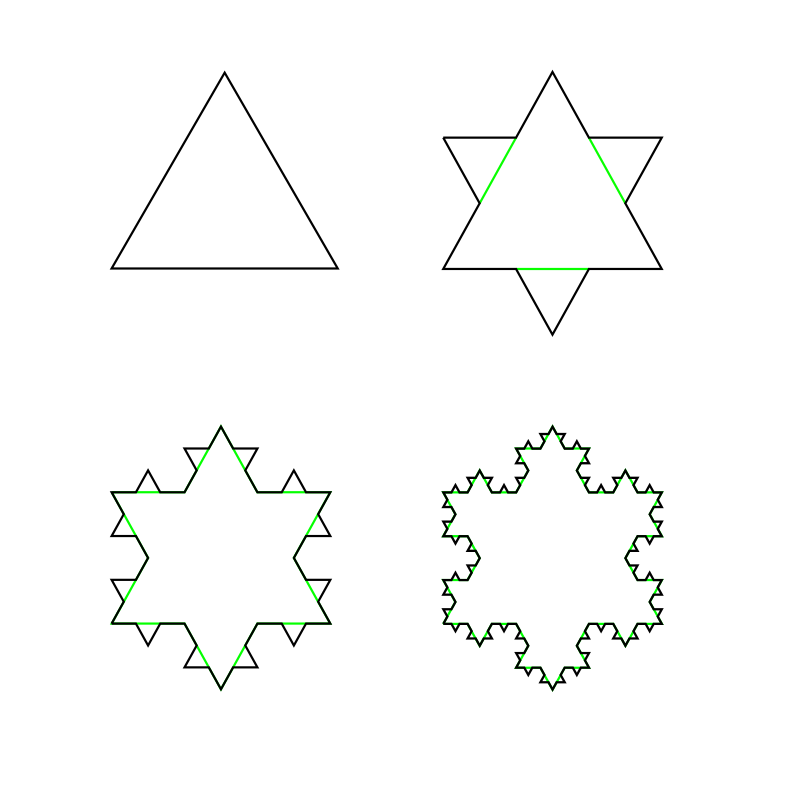
\includegraphics[width=5cm]{include/koch.png}
\end{center}
El copo de nieve de Koch (\url{https://en.m.wikipedia.org/wiki/Koch_snowflake}) es un poligono definido recursivamente.
Dado un poligono (un triangulo por ejemplo), se puede generar el
siguiente poligono asi:
\begin{enumerate}
        \item{Dividir cada linea del poligono en 3 partes exactas.}
        \item{Crear un triangulo nuevo en el espacio abarcado por la linea del medio
        \begin{itemize}
                \item{La longitud de cada linea del triangulo nuevo es la misma que la
                linea del medio.}
        \end{itemize}
        }
\end{enumerate}
Su tarea consiste en definir una funci\'on llamada $\mathtt{snowflake}\ :\ \mathbb{N}\rightarrow
\mathtt{List}\ (\mathbb{R},\mathbb{R})$. Esta funci\'on debe aceptar un numero entero indicando
la cantidad de veces que se repetira la recursion. El valor 0 representa el copo m\'as simple
de Koch (un tirangulo) y numeros mayores a 0 representan la cantidad de repetici\'ones que se
llevaran a cabo en la producci\'on del copo de nieve. El resultado de esta funci\'on es una
lista de parejas de numeros reales ($\mathbf{Float}$) que representan los vertices del copo
de nieve en un plano cartesiano de coordenadas.

\section*{Triangulo de Sierpinski (7pts)}
%%\begin{center}
%%        \includegraphics[width=5cm]{include/sierpinski.jpg}
%%\end{center}
El triangulo de Sierpinski (\url{https://en.wikipedia.org/wiki/Sierpinski_triangle}) es otro fractal generado recursivamente.
El caso base consiste en un triangulo regular. Luego, cada paso recursivo divide cada uno de los triangulos que
conforman el triangulo mediante otro triangulo que cada lado del triangulo esta ubicado en
la mitad de cada una de las lineas del triangulo anterior.
\\\\
Su tarea consiste en definir la funci\'on $\mathtt{sierpinski}\ :\ \mathbb{N}\rightarrow \mathtt{List}\ 
(\mathtt{List}\ (\mathbb{R}, \mathbb{R}))$ la cual debe aceptar un numero entero como parametro y generar
una lista de listas de parejas de numeros reales. La interpretaci\'on de este resultado es que cada
lista de numeros corresponde a uno de los varios triangulos que conforman el triangulo de Sierpinsky.

\section*{Fractal Propio (7pts)}

Los estudiantes tienen la libertad de escoger cual sera el tercer fractal que podra generar su programa.
Puede ser un fractal pre-existente o uno inventado por el estudiante.

\section*{Extra 1: Visualizaci\'on (2.5pts)}

Crear una funci\'on para visualizar los fractales. Cualquier metodo para visualizarlos en HTML
es aceptado pero se recomienda que utilize un Canvas como el que se estudio en clase.

\section*{Extra 2: Controles Web (2.5pts)}

Adicional a la visualizaci\'on grafica de los fractales, crear controles web que permitan
configurar el numero de recursiones que se desea utilizar para cada uno de los fractales asi
como tambi\'en seleccionar que fractal se desea visualizar en un momento dado.

\section*{Extra 3 (2.5pts)}

El estudiante tiene la libertad de implementar funcionalidad o mejoras visuales en su
programa. Puede consultar al catedratico con propuestas para los puntos extra de esta
secci\'on.

\end{document}